% !TEX root = ../ClassicThesis_DEIB.tex

\chapter{Localization and navigation systems in GRAPE} \label{chap:localization}

The studies of \cite{outdoorNavigation}, that analyze main issues in autonomous mobile robot navigation, identify three main problems linked to outdoor autonomous navigation:
\begin{itemize}
	\item the unstructured environment where the actions take place, in opposition to the clear and definite one that is typical in indoor navigation (flat floor, right angles, smooth surfaces)
	\item requirement for multiple sensors, to be aware enough of the surrounding environment, in order to take decisions
	\item moving obstacles, like for example pedestrians or cars in a city road
\end{itemize}
The system developed in the context of \ac{GRAPE} project suffers critically mostly of the first two point listed above. Indeed, the vineyard environment, even if characterized by a certain degree of regularity due to the presence of parallel rows of trees, presents strongly difficulties regarding lack of structure in the terrain configuration (steep, bumpy, clay-rich, muddy, according to the weather conditions and the intrinsic composition and morphology of the terrain) and in the obstacles (non-straight surfaces, different reflectivity and lighting conditions). Moreover, the problem of the fusion of the data coming from the disparates sensors mounted on board of the robot was already addressed from a theoretically point of view in Section \ref{sec:sensorFusion}, and it's the major component in the localization system of the robot. Note that, being our robot an agricultural \ac{UGV}, the problem of moving obstacles is not particularly relevant, since they are most likely to be humans, aware of the robot presence and functionalities, or at most small wild animals (\textit{e.g.} foxes, hares, cats) in remote cases, that however have a very low probability of approaching the Husky base.

In the next section we are going to analyze with detail the configuration of both the odometry and navigation systems running on the \ac{UGV}. It will be clear that both the problems, even if eventually solved using \textit{off-the-shelf} solutions, were all but simple problems and required a real understanding of the numerous problems that arose.

\section{odometry system}\label{sec:odometrySystem}

The configuration of a robust odometry system for vineyard navigation has been a workpoint since the beginning of the project, because of the strong instability of the wheel odometry. To the reasons mentioned at the beginning of the Chapter, we recall also the intrinsic lack of precision due to skid steering kinematics of the Husky base.
We can describe the search for a robust odometry system for the \ac{UGV} in three main phases:
\begin{enumerate}
	\item As hinted in Section \ref{sec:sensorFusion}, in the early phases of \ac{GRAPE} project, the designated sensor fusion framework was \textbf{ROAMFREE}, that had given proof of good functioning in the past (see Section \ref{sec:sensorFusion} for precise references). ROAMFREE platform provides multi-sensors pose tracking and it is designed to be flexible and to adapt to every kind of mobile robotic platform. The tracking module is based on Gauss-Newton minimization of the error functions associated to sensor readings. In order to improve generality, physical sensors are abstracted with \textit{logical sensors}, which are characterized only by the type of the proprioceptive measurement they produce. An other ROAMFREE module provides instead self-calibration modules, using error models for each sensor category to provide on-line correction of the common sources of distortion, bias and noise (\textit{e.g.} hard and soft magnetic distortion, sensor displacement or misalignment). The usage of ROAMFREE framework was specified in the project proposal, thus it was of course the default choice for the sensor fusion framework in the first \textit{integration week} in Garriguella (ES), before this thesis work beginning. The \ac{ROS} implementation of ROAMFREE is still experimental, but a configuration was identified to fit the requirements. Unfortunately, the same configuration turned out to perform poorly during the second integration week in Casciana Terme (IT). This was caused by concurrence of:
	\begin{itemize}
		\item presence of a significant slope in the vineyard, in opposition to the flat (even if bumpy) terrain in Garriguella
		\item difficulty to handle inaccurate configuration of magnetometer and \ac{IMU}
		\item overall trickiness in the configuration procedure, being ROAMFREE integration with \ac{ROS} still experimental
	\end{itemize}
	The low performances of this framework in our situation were pretty clear, so we opted for a more tested and consolidated solution, \textbf{Robot Localization}.
	
	\item The configuration of Robot Localization requires, for each fused sensor, a configuration vector, in which specify which components of the input estimate should be fused into the final pose estimate. Note that the the configuration vector is given in the \textit{frame\_id} of the input message: for example, consider a velocity sensor that produces a \textit{geometry\_msgs/TwistWithCovarianceStamped} message with a \textit{frame\_id} of \\ \textit{velocity\_sensor\_frame}. If we assume that the transform would convert $X$ velocity in the \textit{velocity\_sensor\_frame} to $Z$ velocity in the \textit{base\_link\_frame}. To include the $\dot{X}$ data from the sensor into the filter, the configuration vector should set the $\dot{X}$ velocity value to true, and not the $\dot{Z}$ velocity value. In table \ref{tab:robotLocalizationConfig} you can see the configuration vectors for the sensors taken as input from Robot Localization. Note that, for example, GPS only gives a contribute about $x$ and $y$, since the altitude estimation of GPS is often not precise, and it provides no information about the robot orientation. Our configuration of Robot Localization relied on \textbf{two} different \ac{EKF} nodes in cascade:
	\begin{itemize}
		\item a \textit{local} localization node, that fuses continuous data, and estimates the position and orientation of the \textit{base\_link} frame of the robot inside the \textit{odom} frame \textit{i.e.} the frame fixed in the initial position of the robot. In other words, the task of the node is to publish \textit{odom} $\rightarrow$ \textit{base\_link tf} transform (see Section \ref{sec:tf} for recall). 
		\item a \textit{global} localization node, that also fuses low frequency sensors \textit{i.e.} GPS, and estimate the estimates the position and orientation of \textit{odom} frame inside \textit{map} frame. The \textit{map} $\rightarrow$ \textit{odom} trasfomation "adjusts" the position of frame \textit{odom} in order to contextualize the position of the \ac{UGV} inside the map. Otherwise, the robot pose would be tracked only with respect to its initial position (origin of \textit{odom} frame), but no positioning inside a map would be provided.
 	\end{itemize}
In Figure \ref{fig:cascadeRobotLocalization} you can see the computation graph of the aforementioned odometry system: you can observe that:
	\begin{itemize}
		\item both nodes write on \textit{tf} topic the respective \textit{tf} transform
		\item the local node takes \ac{IMU} (\textit{/imu/data} topic) and wheels (\textit{/husky\_velocity\_controller/odom} topic) estimate for the fusion task
		\item the global node takes as input the pose estimate from GPS (\textit{/odometry\_gps} topic), and the pose estimate from the local node (\textit{/odometry/ekf\_local\_filtered} topic), to implement the cascade.
	\end{itemize}

	\item Even if the cascade produced a pretty precise odometry estimate, the odometry computation was shrunk in a single \ac{EKF} node for two main reasons:
	\begin{itemize}
		\item as we'll describe in Section \ref{sec:navigationSystem}, the navigation system switched to a mapless configuration, so the \textit{tf} transform  \textit{map} $\rightarrow$ \textit{odom} became useless
		\item the \ac{EKF}s cascade configuration led to a short delay in the odometry computation (\textasciitilde200-300 ms). This caused some problems with the obstacle detection implemented through \ac{LIDAR} data, that are processed with negligible delay, and especially when the robot moved from the end of a row of vines to the beginning of another one. 
	\end{itemize}
\end{enumerate}

\setlength\tabcolsep{3pt}
\begin{table}[tb]
\footnotesize
\centering
\begin{tabularx}{0.85\textwidth}{X|XXXXXXXXXXXXXXXX}
\hline
\toprule
\tableheadline{l}{ }  &
\tableheadline{r}{$x$}  &
\tableheadline{r}{$y$}  &
\tableheadline{r}{$z$}  &
\tableheadline{r}{$\psi$}  	&
\tableheadline{r}{$\theta$}  	&
\tableheadline{r}{$\phi$}	&
\tableheadline{r}{$\dot{x}$}  	&
\tableheadline{r}{$\dot{y}$}  		&
\tableheadline{r}{$\dot{z}$}   	&
\tableheadline{r}{$\dot{\psi}$}   		&
\tableheadline{r}{$\dot{\theta}$}	&
\tableheadline{r}{$\dot{\phi}$}   		&
\tableheadline{r}{$\dot{\theta}$}   	&
\tableheadline{r}{$\ddot{x}$}   		&
\tableheadline{r}{$\ddot{y}$}  		 &
\tableheadline{r}{$\ddot{z}$}   		\\
\midrule
\tablefirstcol{l}{Wheels}
&  \ding{51} & \ding{51}  & \ding{51} &  &  & \ding{51} &\ding{51}  &\ding{51}  &\ding{51}  &  &  &  &  &  &  & \\
\midrule
\tablefirstcol{l}{IMU}
&  &   & & \ding{51} &  \ding{51} &  \ding{51}&  &  & &  & \ding{51} &\ding{51}  & \ding{51} & \ding{51} &  & \\
\midrule
\tablefirstcol{l}{GPS points}
&  \ding{51}& \ding{51}  &  &  &  &  &  &  &  &  &  &  &  &  &  & \\
\bottomrule
\end{tabularx}
\caption[Robot localization configuration]{Configuration vectors for the sensors fused for odometry estimation with Robot Localization.}
\label{tab:robotLocalizationConfig}
\end{table}
\setlength\tabcolsep{6pt}

\begin{figure}
	\centering
	\subfloat[]{%
		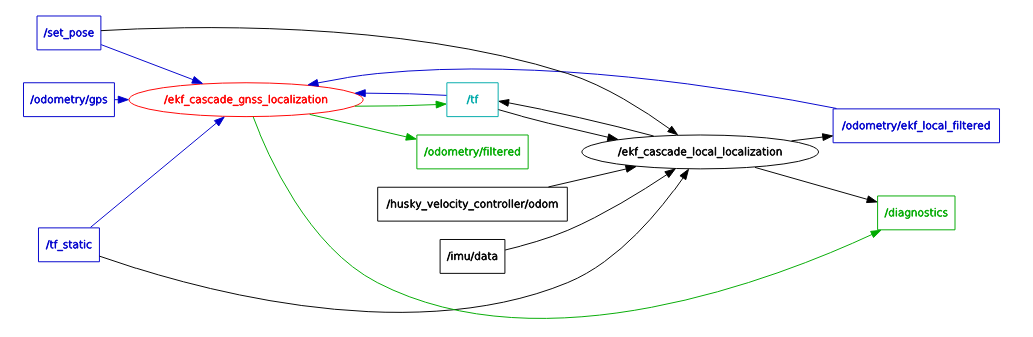
\includegraphics[width=0.9\textwidth]{Images/localization/cascadeGNSSgraph.png}
		\label{fig:cascadeGNSSgraph}} \\
	\subfloat[]{%
		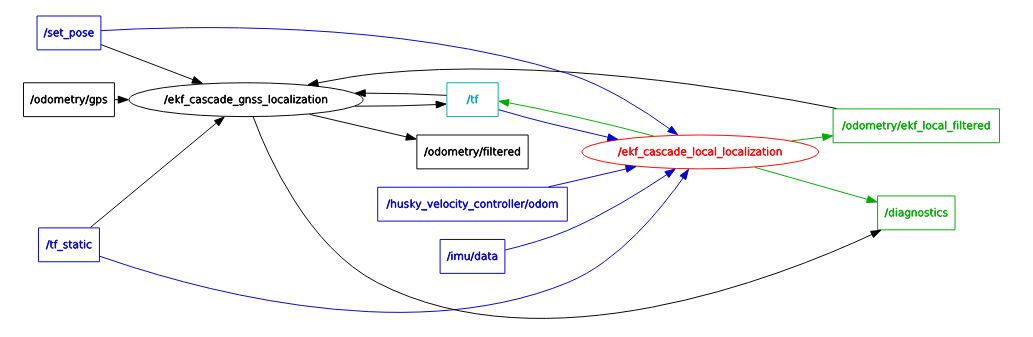
\includegraphics[width=0.9\textwidth]{Images/localization/cascadeLocalGraph.png}
		\label{fig:cascadeLocalGraph}}
	\caption{\textit{Computation graph of the cascade of Robot Localization nodes; in blue, the input topics, and in green the output topic, of the nodes highlighted in red.}}
	\label{fig:cascadeRobotLocalization}
\end{figure}


\section{navigation system}\label{sec:navigationSystem}

We already anticipated in Section \ref{sec:navigationStack} that the reference navigation framework is \textbf{Move Base}, that is an \textit{off-the-shelf} \ac{ROS} software stack for autonomous navigation (see Figure \ref{fig:navStack} for a graphical representation of the main software modules of Move Base). Since, as already stated, this framework usually provides very stable autonomous navigation in indoor mapped environment, the first attempt was to shift the same configuration in the vineyard environment. In this Section we'll show the evolution of the navigation system from this initial configuration to the final one.

\subsection{Mapped navigation with amcl}
Before the robot could be able to navigate the vineyard, this configuration required a preparatory \textit{mapping} phase; in particular, this is a \ac{SLAM} problem, that is the computational problem of constructing or updating a map of an unknown environment, while simultaneously keeping track of an agent's (the \ac{UGV}) location within it. Note that \textit{localization} is a different task with respect to \textit{odometry estimate}, because the first aims to estimate the position of the robot inside a map, while the latter aims to estimate the position of the robot with respect to a reference frame. Even if it is a \textit{chicken-and-egg} problem (localization is easy in a known map, under some assumptions, mapping is easy if the robot position is assumed known), several algorithms exist that solve, even if approximately, the \ac{SLAM} problem. In the early phases of \ac{GRAPE}, previous to this thesis work and described in \cite{grapeAltroPaper}, three different \ac{SLAM} algorithms were tested in our specific environment: \textit{Gmapping}, \textit{Google's Cartographer} and \textit{KartoSLAM}, and \textbf{Gmapping} algorithm was selected because of its performance and reactivity. In Figure \ref{fig:vineyardMaps} you can see some of the maps produced during the first integration week in Garriguella (ES), with these algorithms. The accomplished accuracy of the maps was satisfying, but actually a lot of problems occurred in the main phase, that is the autonomous navigation of the robot in the mapped environment. As you can see in Figure \ref{fig:navStack}, an optional node called \textbf{amcl} exists, that provides a \ac{ROS} implementation of \ac{AMCL} \parencite{amcl}. \ac{AMCL} is a localization algorithm, based on a particle filter to represent the probability distribution over the possible states. A single particle represent a hypothesis about the real pose of the robot in the environment (see Figure \ref{fig:amclAlgoritmo}). Since \ac{AMCL} is a genetic algorithm \parencite{geneticAlgorithm}, each particle is assigned a weight that correspond to the probability that, had it been at the state of the particle, it would perceive what its sensors have actually sensed. Formally:

In particular, \textit{amcl} package is only capable to deal with laser scans as sensor input

\begin{figure}
	\centering
	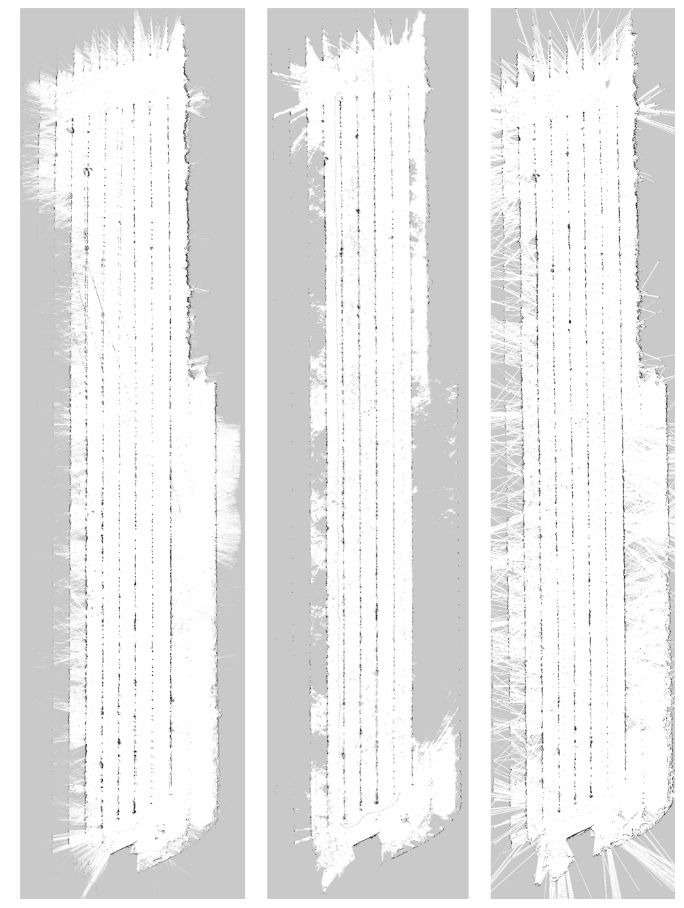
\includegraphics[width=0.7\textwidth]{Images/localization/vineyardMaps.png}
	\caption{\textit{Mapping process output, executed in Mas Llunes vineyard; using Google's Cartographer (left), Gmapping (center), and KartoSLAM (right).}}
	\label{fig:vineyardMaps}
\end{figure}

\begin{figure}
	\centering
	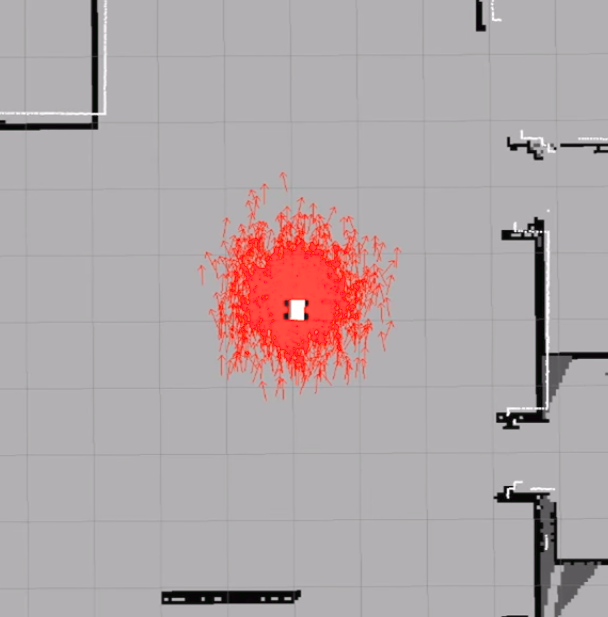
\includegraphics[width=0.7\textwidth]{Images/localization/amcl.png}
	\caption{\textit{Mapping process output, executed in Mas Llunes vineyard; using Google's Cartographer (left), Gmapping (center), and KartoSLAM (right).}}
	\label{fig:amclAlgoritmo}
\end{figure}

inizialmente, map: molto ripetitiva, grossi problemi con amcl;  inoltre problema perché sto scemo prova a passare in mezzo ai filari. Quindi virtual fences, inflated in global map, non inflated in local. Allora visti problemi di amcl e mappa, proviamo mapless: mappa bianca in cui mettere solo fences, e poi local costmap dice la sua. In questo modo le virtual fences sono usate per global planning. 
Dopo lo switch, provato a reintegrare la mappa usando amcl come input al nodo gnss di rob loc. Tuttavia, per motivi da capire non funzia molto bene. Problemi con il local planner dwa (tende a incastrarsi negli angoli), passaggio a elastic band.




\begin{algorithm}
\caption{Monte Carlo Localization($X_{t-1},u_t,z_t$)}\label{alg:mcl}
\begin{algorithmic}[1]
\State $\overline{X}_t=X_t=\emptyset$
\State for $m=1$ to $M$: 
\Indent
	\State $x^{[m]}_t=$ motion\_update($u_t,x^{[m]}_{t-1}$)
	\State $w^{[m]}_t=$ sensor\_update($z_t,x^{[m]}_{t}$)
	\State $\overline{X}_t = {X}_t + \big \langle x^{[m]}_t, w^{[m]}_t \big \rangle$
\EndIndent
\State endfor
\State for $m=1$ to $M$: 
\Indent
	\State draw $x^{[m]}_t$ from $\overline{X}_t$ with probability $\propto w^{[m]}_t$
	\State $X_t=X_t+x^{[m]}_t$
\EndIndent
\State endfor
\State return $X_t$
\end{algorithmic}
\end{algorithm}



Localization Chapter SKETCH:
\begin{itemize}
	\item problemi avuti: mappa molto ripetitiva, il robot tenta di passare attraverso i filari, odometria delle ruote poco affidabile dato il terreno, problemi con amcl
	\item virtual obstacles: cenni (perché non l'ho fatto io) e immagini
	\item configurazione di robot localization, con i sensori usati (ruote+imu+gps)
	\item non sappiamo ancora quale sarà la soluzione utilizzata alla fine tra la versione mapless e amcl integrato con robot\_localization (o eventuali altre soluzioni che salteranno fuori). Una volta che è stata presa una decisione, presentare quella come soluzione definitiva e spiegare perché l'altra è stata giudicata meno efficace
\end{itemize}

